\documentclass[b5paper,10pt,twoside]{book}
\usepackage[inner=1.5cm,outer=2cm,tmargin=1.5cm,bmargin=2cm]{geometry}

\usepackage[utf8]{inputenc}
\usepackage[spanish]{babel}
\usepackage{subfiles}
\usepackage{fancyhdr}
\usepackage[nottoc]{tocbibind}
\usepackage[square,numbers]{natbib}



\usepackage{graphicx}
\graphicspath{ {images/} }
\bibliographystyle{abbrvnat}

\pagestyle{fancy}
\fancyhf{}
\fancyhead[L]{Diario de un superviviente}

\fancyfoot[LE,RO]{\thepage}

\title{Proyecto Fin carrera}
\author{Fernando Santa Olaya Rodríguez \\
	\and 
	Rubén Toquero González}

\date{Septiembre, 2015}


\begin{document}
	\maketitle
	

	\chapter*{Agradecimientos}

	
	\textit{A pepito porque lo quiero con locura blabla bla\\
		Fernando Santa Olaya Rodríguez\\\\\\
		Quiero agradecer a mi familia todo el apoyo que me han dado durante todos estos años, a los que están y a los que ya no están, a los que dedico este trabajo por razones obvias.\\\\
		Tambíen quiero agradecer al tutor Fernando de Prada Moraga toda la paciencia que ha tenido con nosotros, nos ha comprendido y nos ha ayudado a llevar a cabo esta necesaria tarea.\\
		A mi novia, que es la que me ha sufrido la mayor parte del tiempo, todavia me resulta incomprensible que me siga aguantando despues de tantos años.\\
		Por último agradezco a los profesores de esta escuela sus enseñanzas (espero que bien aprovechadas por mi parte) y a todos aquellos con los que he compartido mi tiempo en mi paso por esta etapa de mi vida que aquí se cierra.\\
		Rubén Toquero González} 
	

	\chapter*{Resumen}
	 	El presente proyecto implementa una aplicación móvil como micro asistente virtual a personas que padezcan la lacra moderna del cáncer y una aplicación en servidor con la que se comunica la app y recopila estadísticas de actividades y estados de animo de los usuarios para su posibles estudios relacionados con la enfermedad. Ademas provee de una plataforma con la que se puede interactuar fácilmente con los usuarios de la misma por un operador de la misma. Todo esto se incluye dentro de la iniciativa "Diario de un superviviente" de la Asociación Española contra el Cáncer.
	 	
	\begin{figure}[h]
		\centering
		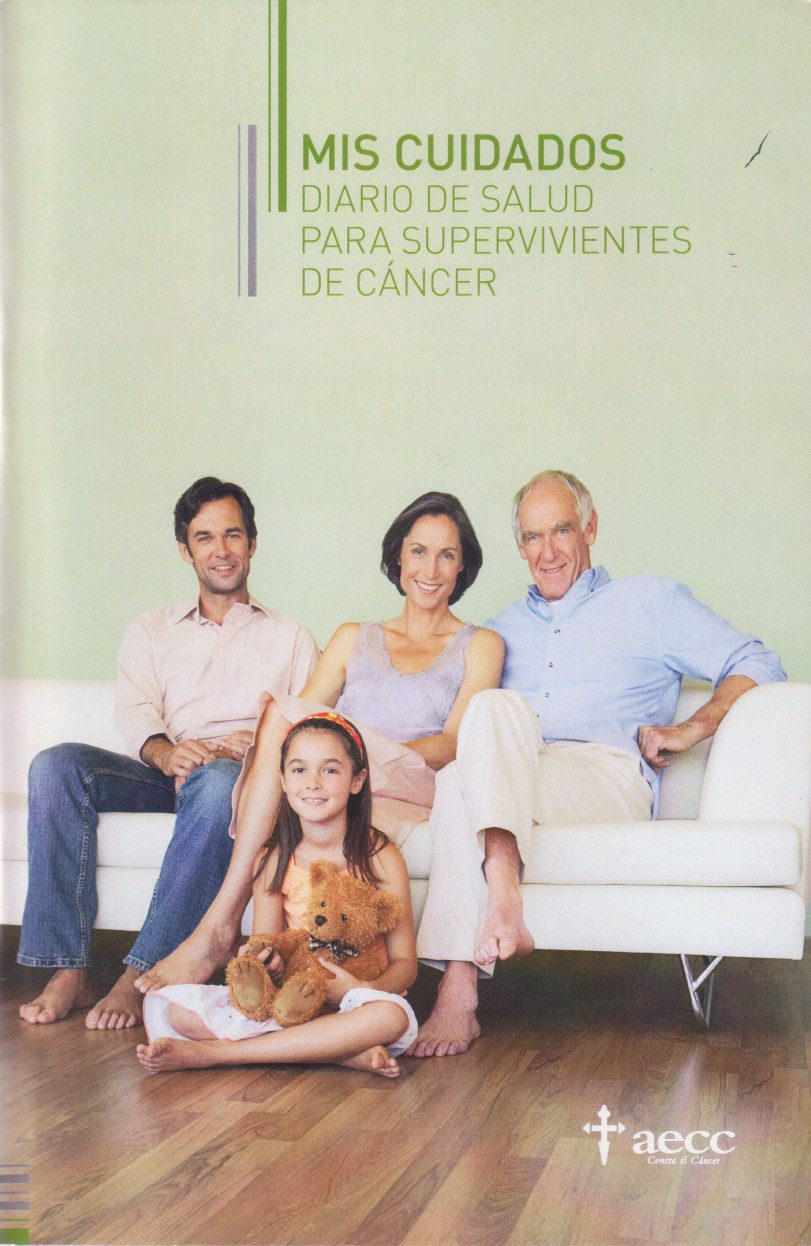
\includegraphics[width=0.25\textwidth]{fotointro}
		\caption{Portada del folleto.}
		\label{fig:mesh1}
	\end{figure}
	 
	\chapter*{Abstract}
	 	This project implents an mobile app wich is an micro virtual assitant for those people who are suffering the modern doom of cancer and on the other hand a server aplication which comunicates with the app on order to acquire data for statistic uses of the data involved with this illnes. Indeed the app serve a platform to interact on an easy way with the users by an operator. All of this is included on the inciative "Survivor's Diary" of the  Asociación Española contra el Cáncer\cite{SHAREESP}
	
	\tableofcontents
	
	\listoffigures
	
	\listoftables
	

	\chapter{INTRODUCCIÓN}
	
	\subfile{./1-Introduccion/introduccion}
	
	\chapter{Visión general del Proyecto}

	\subfile{./2-Vision/vision}
	
	\chapter{Planificación}
	
	\subfile{./3-Planificacion/planificacion}
	
	\chapter{Análisis y Metodología}
	
	\subfile{./4-Analisis/analisis}
	
	\chapter{Diseño}
	
	\subfile{./5-Diseno/diseno}
	
	\chapter{Pruebas}
	
	\subfile{./6-Pruebas/pruebas}
	
	\chapter{Conclusiones y trabajo futuro}
	
	\subfile{./7-Conclusiones/conclusiones}
	
	\chapter{ANEXO I: INSTALACIÓN Y MANUAL DE USUARIO }
		
	\subfile{./8-Anexoi/anexoi}
		
	
		
	\bibliography{bibliography}

\end{document} 